\section{Критическое поведение взаимодействующего блуждания без самопересечений на треугольной решётке}

Основная цель данного раздела - исследование критических свойств модели ISAW на треугольной решётке (далее, TrISAW).
Данная задача решалась ранее, в статье \cite{Privman1986}, с использованием приближений наблюдаемых величин рядями Тейлора.
Полученная оценка точки фазового перехода для TrISAW выписана на таблице \ref{tab:crits}.

В данном разделе мы воспользуемся известными данными о шкалировании радиуса между краями блуждания $R^2_N$:
на основании результатов о невзаимодействующем блуждании без самопересечений \cite{Rensburg2015}, а так же о критическом поведении взаимодействующего блуждания \cite{Duplantier1987} на квадратной решётке,
найдём область конформационного перехода модели и, тем самым, уточним оценку точки фазового перехода.
 

\begin{figure}[h]
\begin{subfigure}{0.49\textwidth}
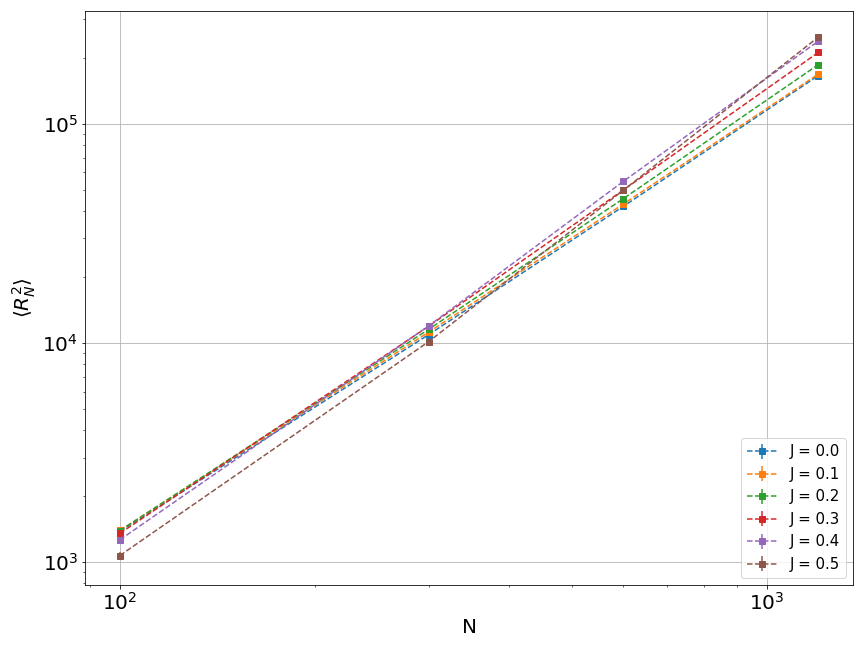
\includegraphics[width=\textwidth]{TrISAW_R2log.png}
\caption{}
\label{fig:TrISAW_R2log}
\end{subfigure}
\hfill
\begin{subfigure}{0.49\textwidth}
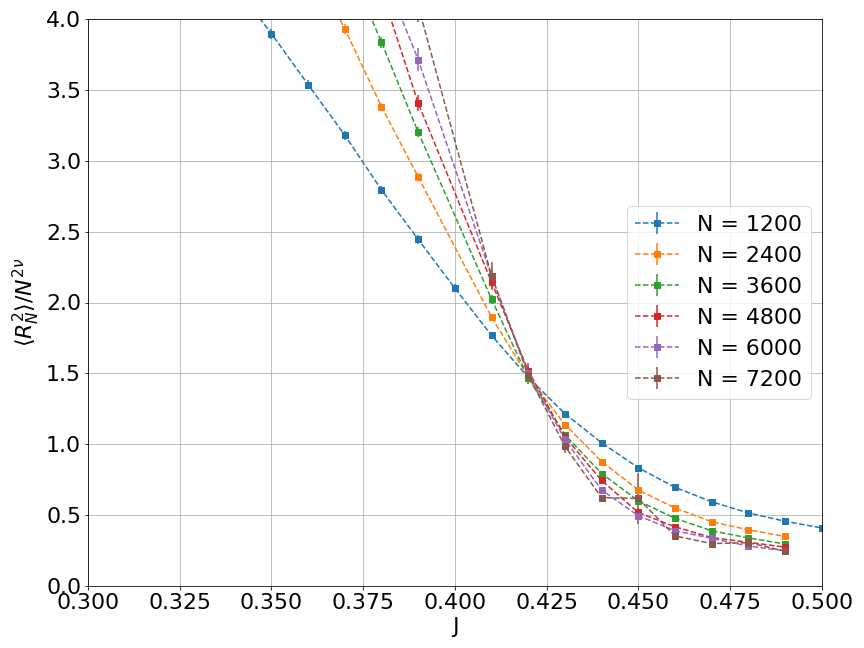
\includegraphics[width=\textwidth]{TrISAW_R2toN2v.png}
\caption{}
\label{fig:TrISAW_R2toN2v}
\end{subfigure}
\caption{а) Расстояние между концами блужданий длины $N$ при $J \in [0.35,0.5]$ в логарифмическом масштабе. 
Для наглядности добавлены линии $N^{2\nu}$, где $\nu = 4/7$ (красная линия) и $\nu=3/4$ (чёрная линия).
б) Отношение расстояния между концами блуждания $R^2_N$ к $N^{2\nu}$, где $\nu=4/7$ при $J \in [0.3,0.5]$}
\end{figure}

На левом рисунке \ref{fig:TrISAW_R2log} изображена зависимость радиуса между концами блуждания TrISAW $R^2_N$ от длины цепочки $N$ в логарифмическом.
При $J < 0.4$ шкалирование радиуса $R^2_N$ - наклон графиков блуждания с соответствующей константой - с ростом длины цепочки приближается к поведению невзаимодействующего блуждания (черная линия с $\nu = 3/4$ \cite{Rensburg2015}).
В области $J \in [0.4, 0.43]$ блуждания приобретает критические свойства, и наклон графиков соответствует красной линии с показателем $\nu=4/7$ \cite{Duplantier1987}.
Дальнейшее увеличение константы $J$ приводит к уменьшению показателя $\nu$ до поведения плотной глобулы.

На правом рисунке эта же величина перешкалирована относительно $N^{2\nu}, \nu = 4/7$ с зависимостью от константы $J$.
Результаты показывают почти идеальное пересечение с точке $J=0.42$, указывая на переход между преобладанием поправок на конечный размер блуждания и усилением шкалирующих свойств величины.

Таким образом, рассматривая конформационный переход модели TrISAW, можно сделать вывод, что фазовый переход модели происходит возле точки $J=0.42$.
Считая погрешностью оценки расстояние между выполненными замерами, итоговая оценка точки фазового перехода модели ISAW на треугольной решётке:

  \begin{equation}
\label{eq:TrISAW_Jc}
	J_c = 0.42(1)
\end{equation}